% LaTeX source for ``Python for Informatics: Exploring Information''
% Copyright (c)  2010-  Charles R. Severance, All Rights Reserved

\chapter{Conditional execution}

\section{Boolean expressions}
\index{boolean expression}
\index{expression!boolean}
\index{logical operator}
\index{operator!logical}

A {\bf boolean expression} is an expression that is either true
or false.  The following examples use the 
operator {\tt ==}, which compares two operands and produces
{\tt True} if they are equal and {\tt False} otherwise:

\beforeverb
\begin{verbatim}
>>> 5 == 5
True
>>> 5 == 6
False
\end{verbatim}
\afterverb
%
{\tt True} and {\tt False} are special
values that belong to the type {\tt bool}; they are not strings:

\index{True special value}
\index{False special value}
\index{special value!True}
\index{special value!False}
\index{bool type}
\index{type!bool}

\beforeverb
\begin{verbatim}
>>> type(True)
<type 'bool'>
>>> type(False)
<type 'bool'>
\end{verbatim}
\afterverb
%
The {\tt ==} operator is one of the {\bf comparison operators}; the
others are:

\beforeverb
\begin{verbatim}
      x != y               # x is not equal to y
      x > y                # x is greater than y
      x < y                # x is less than y
      x >= y               # x is greater than or equal to y
      x <= y               # x is less than or equal to y
      x is y               # x is the same as y
      x is not y           # x is not the same as y
\end{verbatim}
\afterverb
%
Although these operations are probably familiar to you, the Python
symbols are different from the mathematical symbols for the same
operations.  A common error
is to use a single equal sign ({\tt =}) instead of a double equal sign
({\tt ==}).  Remember that {\tt =} is an assignment operator and
{\tt ==} is a comparison operator.   There is no such thing as
{\tt =<} or {\tt =>}.

\index{comparison operator}
\index{operator!comparison}


\section {Logical operators}
\index{logical operator}
\index{operator!logical}

There are three {\bf logical operators}: {\tt and}, {\tt
or}, and {\tt not}.  The semantics (meaning) of these operators is
similar to their meaning in English.  For example,

{\tt x > 0 and x < 10} 

is true only if {\tt x} is greater than 0
\emph{and} less than 10.

\index{and operator}
\index{or operator}
\index{not operator}
\index{operator!and}
\index{operator!or}
\index{operator!not}

{\tt n\%2 == 0 or n\%3 == 0} is true if \emph{either} of the conditions
is true, that is, if the number is divisible by 2 \emph{or} 3.

Finally, the {\tt not} operator negates a boolean
expression, so {\tt not (x > y)} is true if {\tt x > y} is false;
that is, if {\tt x} is less than or equal to {\tt y}.

Strictly speaking, the operands of the logical operators should be
boolean expressions, but Python is not very strict.
Any nonzero number is interpreted as ``true.''

\beforeverb
\begin{verbatim}
>>> 17 and True
True
\end{verbatim}
\afterverb
%
This flexibility can be useful, but there are some subtleties to
it that might be confusing.  You might want to avoid it until
you are sure you know what you are doing.

\section{Conditional execution}
\label{conditional execution}

\index{conditional statement}
\index{statement!conditional}
\index{if statement}
\index{statement!if}
\index{conditional execution}

In order to write useful programs, we almost always need the ability
to check conditions and change the behavior of the program
accordingly.  {\bf Conditional statements} give us this ability.  The
simplest form is the {\tt if} statement:

\beforeverb
\begin{verbatim}
if x > 0 :
    print 'x is positive'
\end{verbatim}
\afterverb
%
The boolean expression after the {\tt if} statement is
called the {\bf condition}.  We end the {\tt if} 
statement with a colon character (:) and the line(s) 
after the if statement are indented.  

\beforefig
\centerline{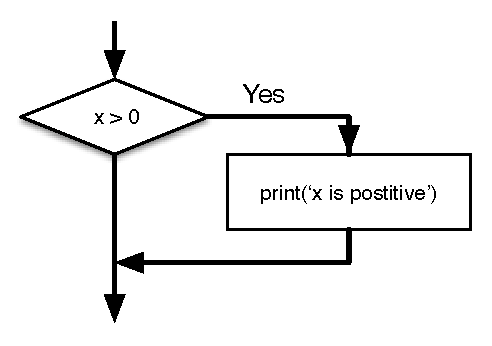
\includegraphics[height=1.75in]{figs2/if.eps}}
\afterfig

If the logical condition is true, then the indented
statement gets executed.  If the logical condition is 
false, the indented statement is skipped.

\index{condition}
\index{compound statement}
\index{statement!compound}

{\tt if} statements have the same structure as function definitions
or {\tt for} loops\footnote{We will learn about functions in Chapter 4
and loops in Chapter 5.}.The statement consists of a header line
that ends with the colon character (:) 
followed by an indented block.  Statements like this are
called {\bf compound statements} because they stretch 
across more than one line.

There is no limit on the number of statements that can appear in
the body, but there must be at least one.
Occasionally, it is useful to have a body with no statements (usually
as a placekeeper for code you haven't written yet).  In that
case, you can use the {\tt pass} statement, which does nothing.

\index{pass statement}
\index{statement!pass}

\beforeverb
\begin{verbatim}
if x < 0 :
    pass          # need to handle negative values!
\end{verbatim}
\afterverb
%
If you enter an {\tt if} statement in the Python interpreter, the prompt will change 
from three chevrons to three dots to indicate you are in the middle of a block of
statements, as shown below:

\beforeverb
\begin{verbatim}
>>> x = 3
>>> if x < 10:
...    print 'Small'
... 
Small
>>>
\end{verbatim}
\afterverb
%

\section{Alternative execution}
\label{alternative execution}

\index{alternative execution}
\index{else keyword}
\index{keyword!else}

A second form of the {\tt if} statement is {\bf alternative execution},
in which there are two possibilities and the condition determines
which one gets executed.  The syntax looks like this:

\beforeverb
\begin{verbatim}
if x%2 == 0 :
    print 'x is even'
else :
    print 'x is odd'
\end{verbatim}
\afterverb
%
If the remainder when {\tt x} is divided by 2 is 0, then we
know that {\tt x} is even, and the program displays a message to that
effect.  If the condition is false, the second set of statements is
executed.  

\beforefig
\centerline{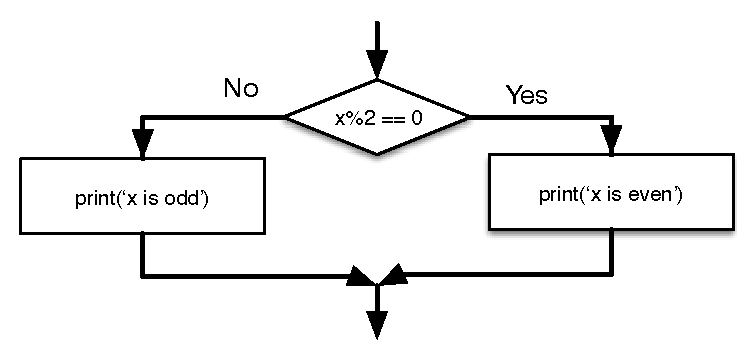
\includegraphics[height=1.75in]{figs2/if-else.eps}}
\afterfig

Since the condition must either be true or false, exactly one of
the alternatives will be executed.  The alternatives are called
{\bf branches}, because they are branches in the flow of execution.

\index{branch}



\section{Chained conditionals}
\index{chained conditional}
\index{conditional!chained}

Sometimes there are more than two possibilities and we need more than
two branches.  One way to express a computation like that is a {\bf
chained conditional}:

\beforeverb
\begin{verbatim}
if x < y:
    print 'x is less than y'
elif x > y:
    print 'x is greater than y'
else:
    print 'x and y are equal'
\end{verbatim}
\afterverb
%
{\tt elif} is an abbreviation of ``else if.''  Again, exactly one
branch will be executed.  

\beforefig
\centerline{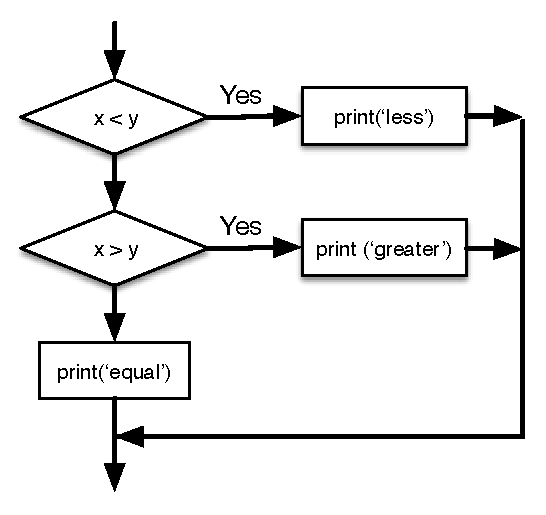
\includegraphics[height=3.00in]{figs2/elif.eps}}
\afterfig

There is no limit on the number of {\tt
elif} statements.  If there is an {\tt else} clause, it has to be
at the end, but there doesn't have to be one.

\index{elif keyword}
\index{keyword!elif}


\beforeverb
\begin{verbatim}
if choice == 'a':
    print 'Bad guess'
elif choice == 'b':
    print 'Good guess'
elif choice == 'c':
    print 'Close, but not correct'
\end{verbatim}
\afterverb
%
Each condition is checked in order.  If the first is false,
the next is checked, and so on.  If one of them is
true, the corresponding branch executes, and the statement
ends.  Even if more than one condition is true, only the
first true branch executes.  


\section{Nested conditionals}
\index{nested conditional}
\index{conditional!nested}

One conditional can also be nested within another.  We could have
written the three-branch example like this:

\beforeverb
\begin{verbatim}
if x == y:
    print 'x and y are equal'
else:
    if x < y:
        print 'x is less than y'
    else:
        print 'x is greater than y'
\end{verbatim}
\afterverb
%
The outer conditional contains two branches.  The
first branch contains a simple statement.  The second branch
contains another {\tt if} statement, which has two branches of its
own.  Those two branches are both simple statements,
although they could have been conditional statements as well.

\beforefig
\centerline{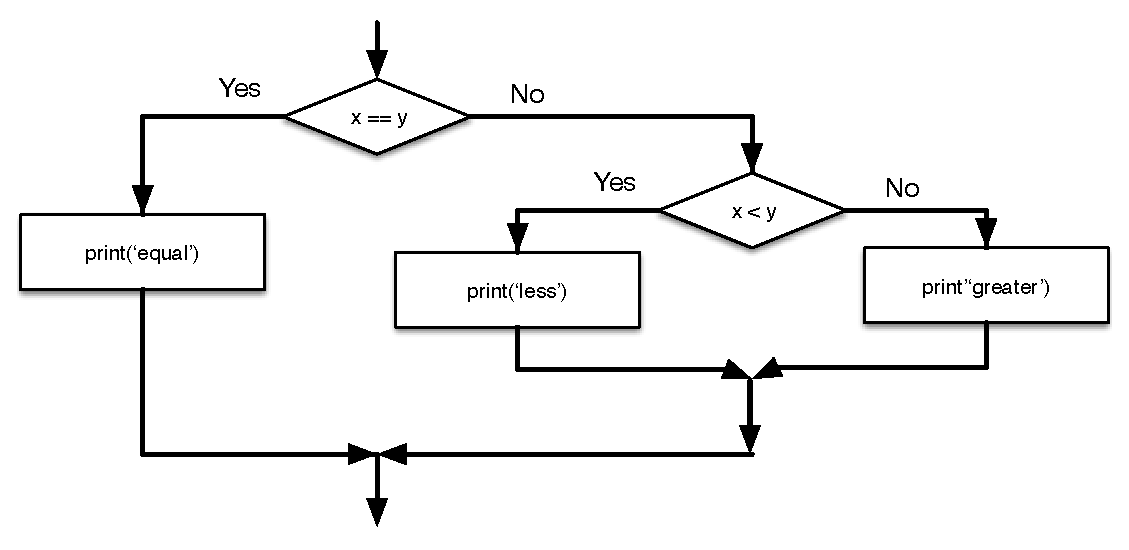
\includegraphics[height=2.50in]{figs2/nested.eps}}
\afterfig

Although the indentation of the statements makes the structure
apparent, {\bf nested conditionals} become difficult to read very
quickly. In general, it is a good idea to avoid them when you can.

Logical operators often provide a way to simplify nested conditional
statements.  For example, we can rewrite the following code using a
single conditional:

\beforeverb
\begin{verbatim}
if 0 < x:
    if x < 10:
        print 'x is a positive single-digit number.'
\end{verbatim}
\afterverb
%
The {\tt print} statement is executed only if we make it past both
conditionals, so we can get the same effect with the {\tt and} operator:

\beforeverb
\begin{verbatim}
if 0 < x and x < 10:
    print 'x is a positive single-digit number.'
\end{verbatim}
\afterverb


\section{Catching exceptions using try and except}
\label{catch1}

Earlier we saw a code segment where we used the \verb"raw_input" and
{\tt int} functions to read and parse an integer number entered by
the user.  We also saw how treacherous doing this could be:

\beforeverb
\begin{verbatim}
>>> speed = raw_input(prompt)
What...is the airspeed velocity of an unladen swallow?
What do you mean, an African or a European swallow?
>>> int(speed)
ValueError: invalid literal for int()
>>>
\end{verbatim}
\afterverb
%
When we are executing these statements in the Python interpreter, 
we get a new prompt from the interpreter, think ``oops'', and move 
on to our next statement.  

However if you place this code in a 
Python script and this error occurs, your script immediately 
stops in its tracks with a traceback.  
It does not execute the following statement. 
\index{traceback}

Here is a sample program to convert a Fahrenheit temperature 
to a Celsius temperature:
\index{fahrenheit}
\index{celsius}
\index{temperature conversion}

\beforeverb
\begin{verbatim}
inp = raw_input('Enter Fahrenheit Temperature:')
fahr = float(inp)
cel = (fahr - 32.0) * 5.0 / 9.0
print cel
\end{verbatim}
\afterverb
%
If we execute this code and give it invalid input, it simply fails
with an unfriendly error message:

\beforeverb
\begin{verbatim}
python fahren.py 
Enter Fahrenheit Temperature:72
22.2222222222

python fahren.py 
Enter Fahrenheit Temperature:fred
Traceback (most recent call last):
  File "fahren.py", line 2, in <module>
    fahr = float(inp)
ValueError: invalid literal for float(): fred
\end{verbatim}
\afterverb
%
There is a conditional execution structure built into 
Python to handle these types of expected and unexpected
errors called ``try / except''.  The idea of {\tt try}
and {\tt except} is that you know that some sequence
of instruction(s) may have a problem and you want to 
add some statements to be executed if an error occurs.
These extra statements (the except block) are ignored
if there is no error.

You can think of the {\tt try} and {\tt except} feature
in Python as an ``insurance policy'' on a sequence of
statements.

We can rewrite our temperature converter as follows:

\beforeverb
\begin{verbatim}
inp = raw_input('Enter Fahrenheit Temperature:')
try:
    fahr = float(inp)
    cel = (fahr - 32.0) * 5.0 / 9.0
    print cel
except:
    print 'Please enter a number'
\end{verbatim}
\afterverb
%

Python starts by executing the 
sequence of statements in the 
{\tt try} block.  If all goes
well, it skips the {\tt except} block and proceeds.  If an
exception occurs in the {\tt try} block, 
Python jumps out of the {\tt try} block and
executes the sequence of statements in the {\tt except} block.

\beforeverb
\begin{verbatim}
python fahren2.py 
Enter Fahrenheit Temperature:72
22.2222222222

python fahren2.py 
Enter Fahrenheit Temperature:fred
Please enter a number
\end{verbatim}
\afterverb
%

Handling an exception with a {\tt try} statement is called {\bf
catching} an exception.  In this example, the {\tt except} clause
prints an error message.  In general,
catching an exception gives you a chance to fix the problem, or try
again, or at least end the program gracefully.

\section{Short-circuit evaluation of logical expressions}
\index{short circuit}

When Python is processing a logical expression such as 
{\tt x >= 2 and (x/y) > 2}, it evaluates the expression
from left to right.  Because of the definition of {\tt and},
if {\tt x} is less than 2, the expression {\tt x >= 2} is 
{\tt False} and so the whole expression is {\tt False} regardless
of whether {\tt (x/y) > 2} evaluates to {\tt True} or {\tt False}.

When Python detects that there is nothing to be gained by evaluating
the rest of a logical expression, it stops its evaluation and does
not do the computations in the rest of the logical expression.  
When the evaluation of a logical expression stops because the overall
value is already known, it is called {\bf short-circuiting} 
the evaluation.

\index{guardian pattern}
\index{pattern!guardian}
While this may seem like a fine point, the short-circuit behavior
leads to a clever technique called the {\bf guardian pattern}.  
Consider the following code sequence in the Python interpreter:

\beforeverb
\begin{verbatim}
>>> x = 6 
>>> y = 2
>>> x >= 2 and (x/y) > 2
True
>>> x = 1 
>>> y = 0
>>> x >= 2 and (x/y) > 2
False
>>> x = 6
>>> y = 0
>>> x >= 2 and (x/y) > 2
Traceback (most recent call last):
  File "<stdin>", line 1, in <module>
ZeroDivisionError: integer division or modulo by zero
>>> 
\end{verbatim}
\afterverb
%
The third calculation failed because Python was evaluating {\tt (x/y)}
and {\tt y} was zero, which causes a runtime error.  But the second example
did \emph{not} fail because the first part of the expression {\tt x >= 2} 
evaluated to {\tt False} so the {\tt (x/y)} was not ever executed 
due to the {\bf short-circuit} rule and there was no error.

We can construct the logical expression to strategically place a {\bf guard}
evaluation just before the evaluation that might cause an error as follows:

\beforeverb
\begin{verbatim}
>>> x = 1
>>> y = 0
>>> x >= 2 and y != 0 and (x/y) > 2
False
>>> x = 6 
>>> y = 0
>>> x >= 2 and y != 0 and (x/y) > 2
False
>>> x >= 2 and (x/y) > 2 and y != 0
Traceback (most recent call last):
  File "<stdin>", line 1, in <module>
ZeroDivisionError: integer division or modulo by zero
>>>
\end{verbatim}
\afterverb
%
In the first logical expression, {\tt x >= 2} is {\tt False} so the evaluation
stops at the {\tt and}.  In the second logical expression, {\tt x >= 2} is {\tt True}
but {\tt y != 0} is {\tt False} so we never reach {\tt (x/y)}.

In the third logical expression, the {\tt y != 0} is \emph{after} the 
{\tt (x/y) } calculation so the expression fails with an error.

In the second expression, we say that {\tt y != 0} acts as a {\bf guard}
to insure that we only execute {\tt (x/y)} if {\tt y} is non-zero.


\section{Debugging}
\label{whitespace}
\index{debugging}
\index{traceback}

The traceback Python displays when an error occurs contains
a lot of information, but it can be overwhelming.  The most
useful parts are usually:

\begin{itemize}

\item What kind of error it was, and

\item Where it occurred.

\end{itemize}

Syntax errors are usually easy to find, but there are a few
gotchas.  Whitespace errors can be tricky because spaces and
tabs are invisible and we are used to ignoring them.

\index{whitespace}

\beforeverb
\begin{verbatim}
>>> x = 5
>>>  y = 6
  File "<stdin>", line 1
    y = 6
    ^
SyntaxError: invalid syntax
\end{verbatim}
\afterverb
%
In this example, the problem is that the second line is indented by
one space.  But the error message points to {\tt y}, which is
misleading.  In general, error messages indicate where the problem was
discovered, but the actual error might be earlier in the code,
sometimes on a previous line.

\index{error!runtime}
\index{runtime error}

The same is true of runtime errors.  Suppose you are trying
to compute a signal-to-noise ratio in decibels.  The formula
is $SNR_{db} = 10 \log_{10} (P_{signal} / P_{noise})$.  In Python,
you might write something like this:

\beforeverb
\begin{verbatim}
import math
signal_power = 9
noise_power = 10
ratio = signal_power / noise_power
decibels = 10 * math.log10(ratio)
print decibels
\end{verbatim}
\afterverb
%
But when you run it, you get an error message\footnote{In Python 3.0,
  you no longer get an error message; the division operator performs
  floating-point division even with integer operands.}:

\index{exception!OverflowError}
\index{OverflowError}

\beforeverb
\begin{verbatim}
Traceback (most recent call last):
  File "snr.py", line 5, in ?
    decibels = 10 * math.log10(ratio)
OverflowError: math range error
\end{verbatim}
\afterverb
%
The error message indicates line 5, but there is nothing
wrong with that line.  To find the real error, it might be
useful to print the value of {\tt ratio}, which turns out to
be 0.  The problem is in line 4, because dividing two integers
does floor division.  The solution is to represent signal power
and noise power with floating-point values.

\index{floor division}
\index{division!floor}

In general, error messages tell you where the problem was discovered, 
but that is often not where it was caused.


\section{Glossary}

\begin{description}

\item[body:] The sequence of statements within a compound statement.
\index{body}

\item[boolean expression:]  An expression whose value is either 
{\tt True} or {\tt False}.
\index{boolean expression}
\index{expression!boolean}

\item[branch:] One of the alternative sequences of statements in
a conditional statement.
\index{branch}

\item[chained conditional:]  A conditional statement with a series
of alternative branches.
\index{chained conditional}
\index{conditional!chained}

\item[comparison operator:] One of the operators that compares
its operands: {\tt ==}, {\tt !=}, {\tt >}, {\tt <}, {\tt >=}, and {\tt <=}.

\item[conditional statement:]  A statement that controls the flow of
execution depending on some condition.
\index{conditional statement}
\index{statement!conditional}

\item[condition:] The boolean expression in a conditional statement
that determines which branch is executed.
\index{condition}

\item[compound statement:]  A statement that consists of a header
and a body.  The header ends with a colon (:).  The body is indented
relative to the header.
\index{compound statement}

\item[guardian pattern:] Where we construct a logical expression 
with additional
comparisons to take advantage of the short-circuit behavior.
\index{guardian pattern}
\index{pattern!guardian}

\item[logical operator:] One of the operators that combines boolean
expressions: {\tt and}, {\tt or}, and {\tt not}.

\item[nested conditional:]  A conditional statement that appears
in one of the branches of another conditional statement.
\index{nested conditional}
\index{conditional!nested}

\item[traceback:]  A list of the functions that are executing,
printed when an exception occurs.
\index{traceback}

\item[short circuit:]  When Python is part-way through evaluating a 
logical expression and stops the evaluation because Python 
knows the final value for the expression 
without needing to evaluate the rest of the expression.
\index{short circuit}

\end{description}

\section{Exercises}

\begin{ex}
Rewrite your pay computation to give the employee 1.5 
times the hourly rate for 
hours worked above 40 hours.

\begin{verbatim}
Enter Hours: 45
Enter Rate: 10
Pay: 475.0
\end{verbatim}
\end{ex}

\begin{ex}
Rewrite your pay program using {\tt try} and {\tt except} 
so that your program handles non-numeric input gracefully
by printing a message and exiting the program.
The following shows two executions of the program:

\begin{verbatim}
Enter Hours: 20
Enter Rate: nine
Error, please enter numeric input

Enter Hours: forty
Error, please enter numeric input
\end{verbatim}
\end{ex}

\begin{ex}
Write a program to prompt for a score between 0.0 and 1.0.
If the score is out of range, print an error message.  If the score
is between 0.0 and 1.0, print a grade using the following 
table:

\begin{verbatim}
Score   Grade
>= 0.9     A
>= 0.8     B
>= 0.7     C
>= 0.6     D
< 0.6    F

Enter score: 0.95
A

Enter score: perfect
Bad score

Enter score: 10.0
Bad score

Enter score: 0.75
C

Enter score: 0.5
F
\end{verbatim}

Run the program repeatedly as shown above to test the 
various different values for input.
\end{ex}

